%CHAPTER
\chapter{Patent}
\todo{todo}
základní informace + uložiště dat + info o zdrojích (patentové úřady atp) \newline
\section{Patent vs Užitný vzor}
\section{Patent vs Průmyslový vzor}
\section{Patent vs Ochranná známka}
\section{Patent vs Autorská práva}


%%%%%%%%%%%%%%%%%%%%%%%%%%%%%%%%%%%%%%%%%%%%%%%%%%%%%%%%%%%%

%CHAPTER
\chapter{Databáze}

Databáze je organizovaná kolekce strukturovaných informací nebo dat, která jsou typicky ukládána elektronicky v počítačovém systému. Data / informace lze nazvat jako fakta vztahující se k libovolnému uvažovanému objektu. Typický příklad objektu je člověk, jehož fakta jsou: jméno, věk, výška, váha a mnoho dalších \cite{guru99Database}.\newline
\indent Pro správu dat v databázi a její řízení je potřeba komplexní software, který se nazývá \textbf{Systém Řízení Báze Dat} (SŘBD, anglicky DBMS). SŘBD slouží jako interface mezi samotnou databází a koncovým uživatelem (může být i program), umožňující jak vytěžování a aktualizaci dat, tak i možnosti nastavení záloh a jiných administrativních operací \cite{OracleDB}.
\begin{figure}[h!]
\centering
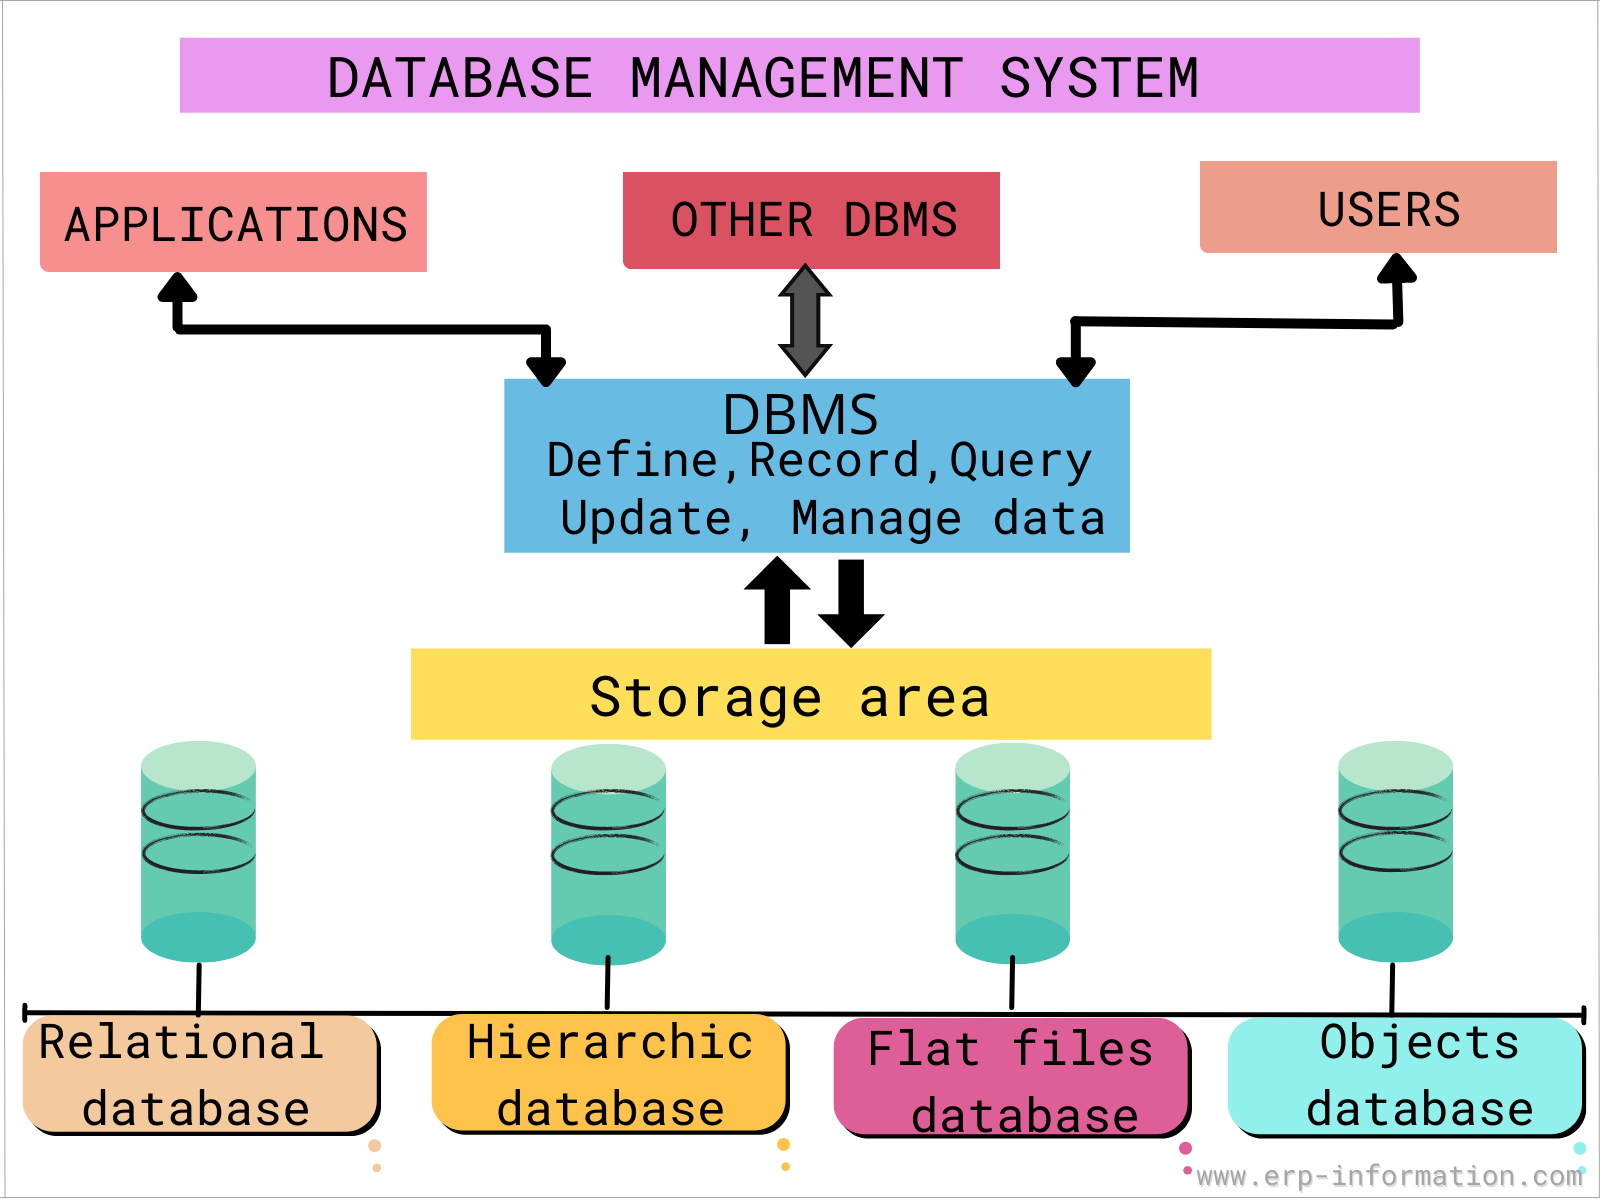
\includegraphics[width=10cm]{img/dbms}
\caption{Systém řízení báze dat}
\label{fig:dbms}
\end{figure}

\section{Komponenty databáze}
Všechny databáze sestávají z pěti základních komponent, nehledě na použitý typ databáze \cite{TechTargetDB, guru99Database}:
\begin{itemize}
\item \textbf{Hardware} - Fyzické stroje (počítače, servery, pevné disky, ...) na kterých běží databázový software.
\item \textbf{Software} - Databázový software poskytuje uživateli / programu kontrolu nad databází. Zahrnuje to samotný databázový software, operační systém, software pro správu sdílení dat mezi uživately a programy pro přístup k datům v databázi.
\item \textbf{Data} - Nezpracované a neorganizované fakty, které je potřeba zpracovat. Administrátor databáze organizuje tyto data a dává jim význam. Data se obecně skládají hlavně z faktů, observací, percepcí, čísel, znaků a mnoho dalších.
\item \textbf{Jazyk} - Typický příklad použití jazyku je přístup k datům, přidávání nových dat, úpravu již existujících dat z databáze. Uživatel / program napíše specifické příkazy v jazyku pro přístup k datům (Database Access Language) a tyto příkazy následně pošle databázi ke zpracování. Více viz kapitola č. \ref{sec:jazyky}.
\item \textbf{Procedury} - Procedura obsahuje předpřipravený seznam příkazů, které se následně vykonávají po zavolání dané procedury. 
\end{itemize}

\section{Jazyky} \label{sec:jazyky}
Databázové jazyky, jinak známé jako dotazovací jazyky, jsou klasifikací programovacích jazyků, které se používají k definování a přístupu k databázím. Pomocí těchto jazyků dokáže uživatel získávat nebo spravovat data v databázích. V dnešní době se jazyky (např. SQL) mohou skládat ze čtyř podjazyků, kdy každý slouží k jinému účelu v rámci vykonávání příkazů \cite{indeedDBLanguage, begginersBookDBLanguage}:
\begin{itemize}
\item \textbf{Data definition language} (DDL) - DDL umí vytvářet jednotlivé komponenty databázového schématu (tabulky, soubory, indexy, ...), které tvoří strukturu reprezentující organizaci dat v databázi. Dostupné příkazy pro jazyk DDL:
	\begin{itemize}
	\item \textbf{CREATE} - Vytvoření nového objektu (tabulka, index, ...).
	\item \textbf{ALTER} - Změna struktury objektu.
	\item \textbf{DROP} - Smazání objektu.
	\item \textbf{RENAME} - Změna názvu objektu.
	\item \textbf{TRUNCATE} - Smazání podobjektů v objektu (např. záznamy v tabulce).
	\end{itemize}
\item \textbf{Data manipulation language} (DML) - DML slouží pro manipulaci s daty, které se nachází v již existující databázi. Dostupné příkazy pro jazyk DML:
	\begin{itemize}
	\item \textbf{SELECT} - Získání záznamů (dat) z tabulky.
	\item \textbf{INSERT} - Vložení nového záznamu (dat) do tabulky.
	\item \textbf{UPDATE} - Úprava existujícího záznamu v tabulce.
	\item \textbf{DELETE} - Smazání záznamu z tabulky.
	\end{itemize}
\item \textbf{Data control language} (DCL) - Pomocí DCL lze kontrolovat přístupy a práva k datům, které jsou uloženy v databázi. Uživateli lze nastavit práva k jednotlivým DML příkazům nad tabulkama / procedurama (např. uživatel bude mít přístup pouze k příkazu SELECT nad tabulkou "TABULKA"). Dostupné příkazy pro jazyk DCL:
	\begin{itemize}
	\item \textbf{GRANT} - Přidání práv uživateli nad danou tabulkou / procedurou. 
	\item \textbf{REVOKE} - Odebrání práv uživateli nad danou tabulkou / procedurou.
	\end{itemize}

\item \textbf{Transaction control language} (TCL) - TCL spravuje transakce v databázi. Transakce obsahuje jeden či více DML příkazů nad tabulkama, které se vykonávají po sobě. Všechny příkazy musí být úspěšně provedeny, aby bylo možné transakci označit za úspěšnou. Ukázka jedné transakce viz obrázek č. \ref{fig:tcl_savepoint}. Dostupné příkazy pro jazyk TCL:
	\begin{itemize}
	\item \textbf{COMMIT} - Potvrzení transakce, změny provedené v transakci jsou permanentní a nejdou vzít zpět.
	\item \textbf{ROLLBACK} - Vezme zpět veškerou práci v aktuální transakci. Lze se vrátit na začátek transakce nebo k SAVEPOINTu.
	\item \textbf{SAVEPOINT} - Nastavení bodu v transakci, ke kterému se lze v budoucnu vrátit pomocí ROLLBACK.
	\end{itemize}

	\begin{figure}[h!]
	\centering
	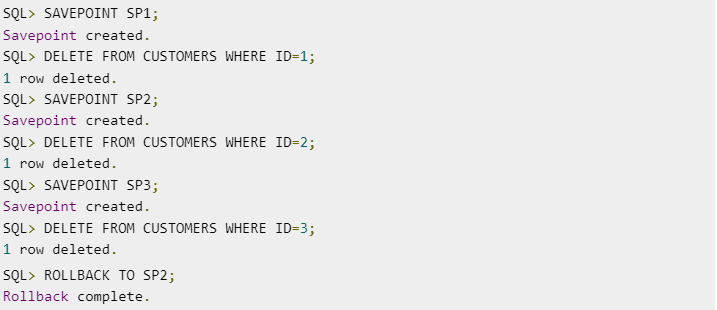
\includegraphics[width=14cm]{img/tcl_savepoint}
	\caption{Ukázka jedné transakce (bez commitu)}
	\label{fig:tcl_savepoint}
	\end{figure}
\end{itemize}

\section{Typy databází}
Lehce popsat\todo{TODO}
\subsection{Relační}
\subsection{Objektově-orientovaná}
\section{Dostupné databáze}
\subsection{MySQL}
\subsection{PostgreSQL}
\cite{TopTenDatabases}Topten\newline
\cite{indeedDBLanguage}\newline
%%%%%%%%%%%%%%%%%%%%%%%%%%%%%%%%%%%%%%%%%%%%%%%%%%%%%%%%%%%%

%\chapter{Docker}
%\todo{todo}
%Popsat docker jako takový - kontejnery, image, docker compose, ...\newline
%\section{Kontejner vs Virtuální stroj}